\chapter{Electric Dipole Moment of Leptons}
\label{ch:leptonEDM}

Following the framework laid out previously, we want to perform EDM calculations on the various leptons.

\section{Experimental Overview}
A brief overview of current experimental bounds and projected future experimental sensitivity is given in \tabref{leptonEDMExperiments}.
\begin{table}[htp]
    \centering
    \begin{adjustbox}{center}
        \begin{small}
            \begin{tabular}{cclcl}
                \toprule
                Lepton & \multicolumn{2}{c}{Current bound (\(e \) cm)} & \multicolumn{2}{c}{Future sensitivity (\(e \) cm)}\\
                \midrule
                Electron & \num{0.41e-29} & JILA~(2023)~\cite{JILA2023eEDM} & & \\
                & \num{1.1e-29} & ACME~(2018)~\cite{ACME2018eEDM} & & \\
                Muon & \num{1.8e-19} & BNL~(2009)~\cite{BNL2009MuonEDM} & \(\sim \num{e-21} \) & FNAL~\cite{Fermilab2016MuonEDM}, J-PARC~\cite{JPARC2019MuonEDM} \\
                & \(\sim \num{2e-20} \) & Pospelov~(2022)~\cite{Pospelov2022MuonEDM} & \(\sim \num{6e-23} \) & PSI~\cite{PSI2021MuonEDM} \\
                Tau & \(\Re\,d_{\tau} = \) \num{-0.62(0.63)e-17} & Belle~\cite{Belle2003TauEDM} & \(\sim \num{e-18}-\num{e-19} \) & Belle II~\cite{BelleII2019Projections} \\
                & & & \(\sim \num{0.7e-19} \) & Bernreuther~\cite{Bernreuther2021TauEDM}\\
                & \(\Im\,d_{\tau} = \) \num{-0.40(0.32)e-17} & Belle~\cite{Belle2003TauEDM} & \(\sim \num{e-18}-\num{e-19} \) & Belle II~\cite{BelleII2019Projections} \\
                & & & \(\sim \num{0.4e-19} \) & Bernreuther~\cite{Bernreuther2021TauEDM} \\
                \bottomrule
            \end{tabular}
        \end{small}
    \end{adjustbox}
\caption{Overview of current bounds and future sensitivities for lepton EDMs.}
\label{tab:leptonEDMExperiments}
\end{table}

As can be seen in the table, the experimental development of electron EDM (eEDM) over the past few years has been remarkably rapid.
Just earlier last year, JILA~\cite{JILA23} has surpassed the previous bound from ACME~\cite{ACME18} and pushed the precision of eEDM down to \(|d_{e}| < 4.1 \times 10^{-30}\) \(e\,\mathrm{cm} \).
It is noteworthy to point out that these eEDM experiments are relatively small in scale, ``tabletop experiments'' even when compared to behemoths like the LHC, which makes the extreme precision achieved all the more impressive.

\section{The Electron}
For the electron, an extensive study of eEDM in {\gthdm} can be found in the 2018 and 2020 papers of Fuyuto, Hou, and Senaha (Refs.~\cite{FHS2018EWBGandEDM,FHS2020EDMCancellation}).
Our investigation on eEDM is essentially an extension of the 2020 paper to a larger parameter space.

\subsection{Cancellation Mechanism}
As mentioned in [CROSSREF], one big motivation for {\gthdm} as a viable model is the fact that \(\order{1} \rho_{tt}\) can drive baryogenesis through \(\lambda_{t}\Im\rho_{tt} \).
However, this same \(\rho_{tt} \), along with \(\rho_{ff} \) for a given fermion \(f \), also generates EDM for said fermion [CROSSREF].
We thus arive at a ``point of tension'' between theory and experiment:
we desire a large \(\rho_{tt} \) for baryogenesis, but need a small \(\rho_{tt} \) to survive precision bounds on various EDMs.
Electron EDM, in particular, is a great ``observable of contention'', since experiments measuring it are the most precise compared to other EDMs.
In an attempt to address this issue, Fuyuto, Hou, and Senaha proposed a ``cancellation ansatz'' between \(\rho_{ee} \) and \(\rho_{tt} \) 
\begin{equation}\label{eq:ansatz}
    \Re\rho_{ee} = -r\frac{\lambda_{e}}{\lambda_{t}}\Re\rho_{tt} \text{, } \quad \Im\rho_{ee} = +r\frac{\lambda_{e}}{\lambda_{t}}\Im\rho_{tt},
  \end{equation}
which facilitates a ``cancellation mechanism'' that allows for small values of eEDM while keeping a \textit{sizeable} \(\rho_{tt} \).
The ``cancellation'' in this mechanism arises from the opposite signs of the \(W \)-loop and the top-loop in the Barr-Zee diagrams.
Referring to~\eqnref{BarrZee-phiG-toploop}~and~\eqnref{BarrZee-cHW-Wloop}, we can see that
\begin{align}
    (d^{\phi G}_{l})_{t} = -&\frac{e\,m_{l}}{(4\pi)^{4}}\sqrt{2}G_{F}\sum_{\phi=h,H,A}\sum_{G=\gamma,Z}(\rho \text{ couplings})(\text{Loop functions}) \\
    (d^{\phi G}_{l})_{W} = +&\frac{e\,m_{l}}{(4\pi)^{4}}\sqrt{2}G_{F}\sum_{\phi=h,H,A}\sum_{G=\gamma,Z}(\rho \text{ couplings})(\text{Loop functions})
\end{align}
thus the effectiveness of such a cancellation is determined by the relationship between the new \(\rho \) couplings and the loop functions of the Barr-Zee diagrams.
In the case of total cancellation, \((d^{\phi G}_{l})_{t} = -(d^{\phi G}_{l})_{W}\), which gives
\begin{equation}\label{eq:exact-cancellation}
    \text{To be added}
\end{equation}
which can be factored into a \(\rho \)-dependent part and a loop-function-dependent part \(r \).
Rearranging~\eqnref{exact-cancellation} thus gives us the form of the cancellation ansatz.
This ansatz signifies two key points.
First, it gives a flavor hierarchy \(|\rho_{ee}|/|\rho_{tt}|\sim\lambda_{e}/\lambda_{t} \) that reflects SM.
Second, it represents a phase lock between \(\rho_{ee} \) and \(\rho_{tt} \).
With our working assumption of Higgs masses, this ansatz results in a ``dip'' in eEDM around the \(r \) value of \(\sim 0.7 \),
which is when complete cancellation occurs between the \(W \)-loop and the top-loop.
This provides a mechanism for the eEDM in {\gthdm} to be small and evade the experimental bounds while not directly modifying \(\rho_{tt} \).

\subsection{Enlarging the Parameter Space}
When revisiting their study, we found the assumptions on the value of \(\rho_{tt} \) to be quite ``conservative'', setting \(\Re\rho_{tt} = \Im\rho_{tt} = -0.1 \) (which equates to \(|\rho_{tt}| = 0.1\sqrt{2} \approx 0.14\)).
We believe that might be due to \textit{playing it safe} under the pressure of the rapid advancements on the experimental front. 
In our study~\cite{HKT2024eEDMnEDM}, we \textit{push against the boundary}, and explore a larger range of \(\rho_{tt} \), up to \(\Re\rho_{tt} = \Im\rho_{tt} = -0.3 \) (\(|\rho_{tt}| = 0.3\sqrt{2} \approx 0.42\)). 
We want to see how big we can keep the parameter space for baryogenesis while still satisfying precision constraints.
As mentioned before, one of the key points of {\gthdm} is the \textit{flavor hierarchy}, illustrated by the \textit{rule of thumb}~\eqnref{ruleofthumb}.
This ``cancellation ansatz'' happens to capture the idea of such a hierarchy pretty well from a numerical standpoint; 
so, for the sake of numerical illustration of the flavor hierarchy, we extend the ansatz to all fermion \(\rho_{ff} \)s, except for the top itself:
\begin{equation}\label{eq:ansatz-extended}
    \Re\rho_{ff} = -r\frac{\lambda_{f}}{\lambda_{t}}\Re\rho_{tt} \text{, } \quad \Im\rho_{ff} = +r\frac{\lambda_{f}}{\lambda_{t}}\Im\rho_{tt}.
\end{equation}
We must reiterate that this is merely a move of convenience, and the actual values of the \(\rho_{ff} \)s need not precisely match this ansatz.
Results are shown in \figref{eEDM}.

\begin{figure}[p]
    \centering
    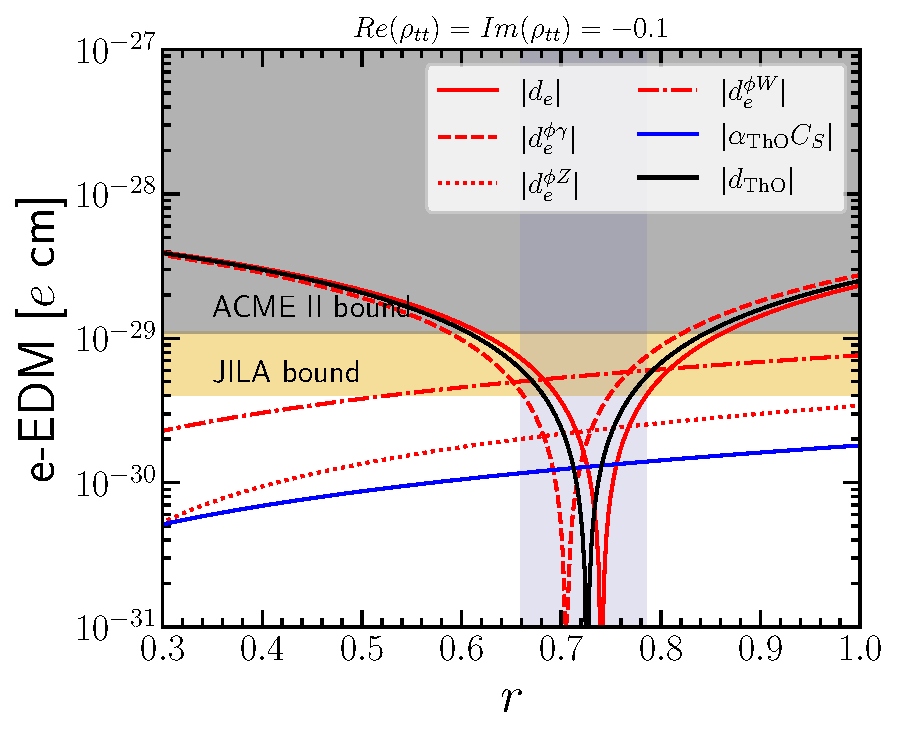
\includegraphics[width=7.95cm,height=5.55cm,angle=-90]{fig2_1.pdf}\\
    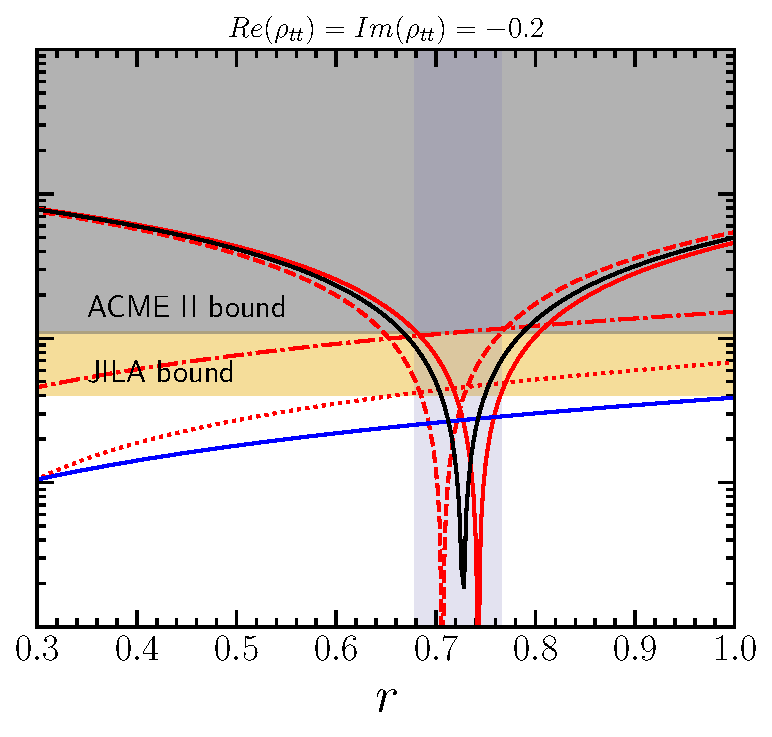
\includegraphics[width=6.95cm,height=5.55cm,angle=-90]{fig2_2.pdf}\\
    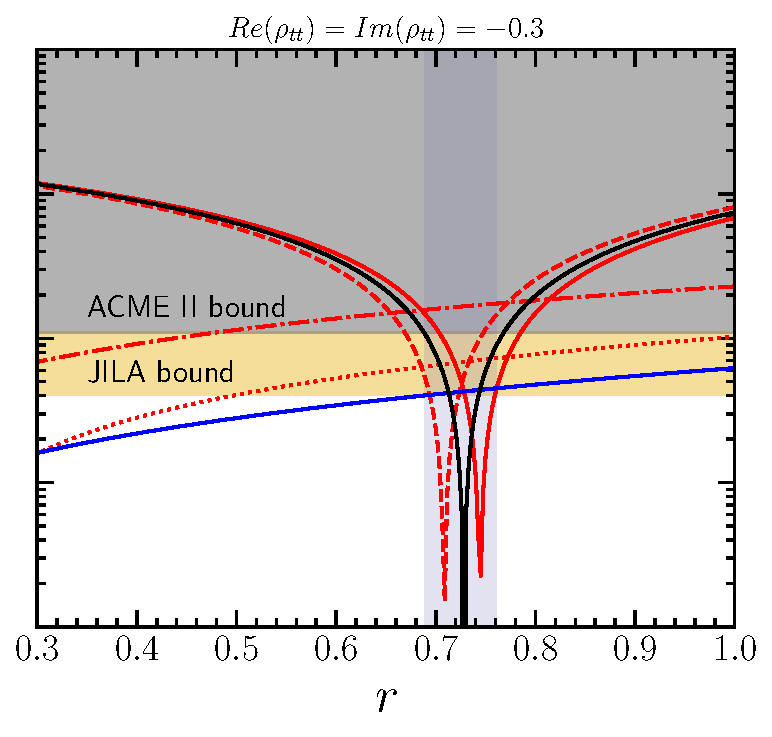
\includegraphics[width=6.95cm,height=5.55cm,angle=-90]{fig2_3.pdf}
    \caption{eEDM v.s. \(r \) for a larger range of \(\rho_{tt} \) with ansatz~Eq.~\eqref{eq:ansatz-extended}. (\(c_{\gamma} = 0.1, m_{H, A, H^+} = 500\,\mathrm{GeV} \))}
    \label{fig:eEDM}
\end{figure}

For the sake of clarity, we have taken a slight liberty in illustrating the range of the purple ``allowed window'' band,
using the left- and right-most curves instead of the left and right side of a given curve.
Nevertheless, the trend we wish to describe is not affected by such.
From our results, it can be seen that as \(|\rho_{tt}| \) increases, the allowed window of the proportionality parameter \(r \) shrinks, yet there is still a decent range of acceptable probable values.
\(\Re\rho_{tt} = \Im\rho_{tt} = -0.1 \) was indeed a conservative representative value, and \(\Re\rho_{tt} = \Im\rho_{tt} = -0.3 \) may still be a viable option in the baryogenesis parameter space.

\section{The Muon}
After the electron, we move on to its slightly heavier cousin, the muon. 
Since the bound on the muon is not as strong, one does not need to resort to the cancellation ansatz immediately.
Instead, we perform a scan of the \(\rho_{tt} \) parameter space for a representative \(\rho_{\mu\mu} \) value, and see how it affects the \(\mu \)EDM.
Results are shown in \figref{muEDM}.

\begin{figure}[p]
    \centering
    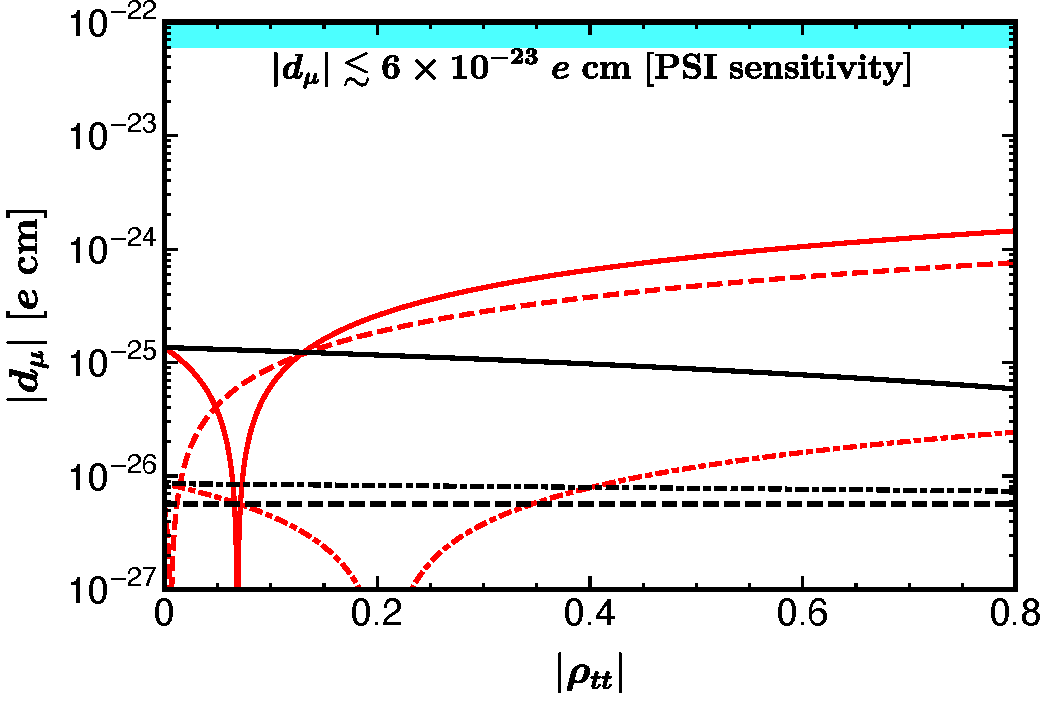
\includegraphics[width=0.7\textwidth]{muEDM.pdf}
    \caption{\(\mu \)EDM results.}
    \label{fig:muEDM}
\end{figure}

We see that there is still a ``cancellation dip'' for the neutral scalar-attached loops, which arises from the opposite signs of the \(W \)-loop and the top-loop.
The details of said cancellation is exactly the same as that of the electron.
Our predicted values for \(\mu \)EDM are still two to three orders of magnitude below the current bounds, so we are eager to see development on the experimental front.
Once the bounds close in, it may also be fruitful to consider the ``cancellation ansatz'' on the muon as well, especially since the leptons share a extra Yukawa matrix \(\rho^{l} \),
which makes it more likely that the \(\rho_{ll} \) might exhibit similar relationships with \(\rho_{tt} \).

\section{The Tau Lepton}
\begin{figure}[p]
    \centering
    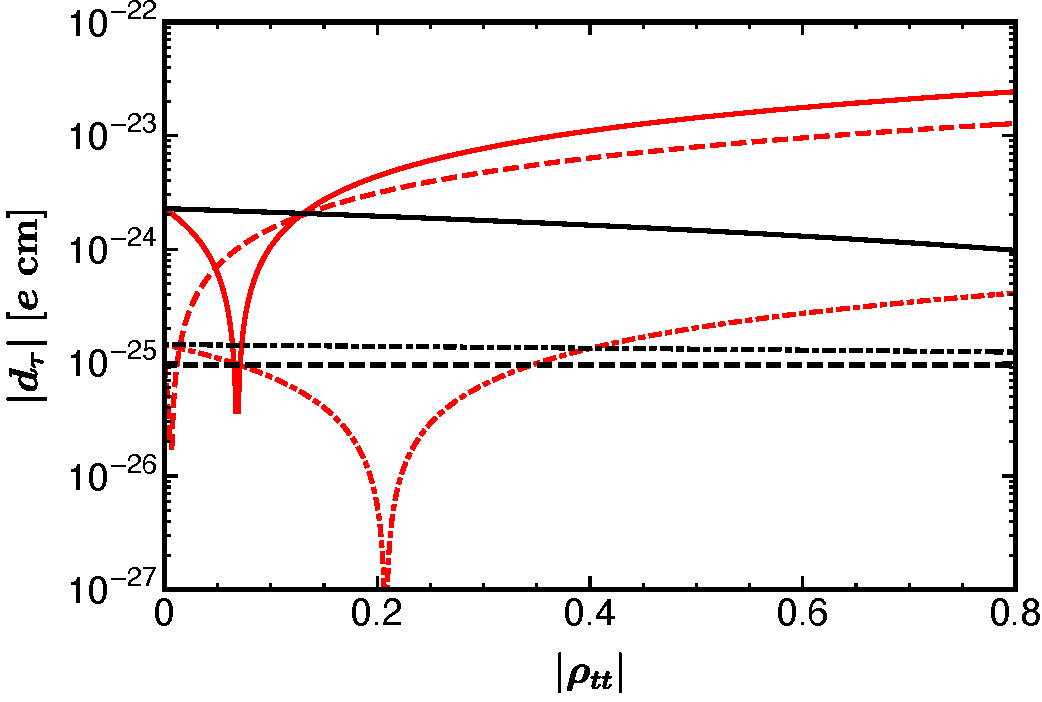
\includegraphics[width=0.7\textwidth]{tauEDM.pdf}
    \caption{\(\tau \)EDM results.}
    \label{fig:tauEDM}
\end{figure}
Lastly, we analyze the heaviest lepton, the tau. 
On the experimental front, the precision of tau EDM (\(\tau \)EDM) measurements are still pretty low.
We perform the same calculations as the muon, with \(\rho_{\mu\mu} = i\lambda_{\mu} \) replaced by \(\rho_{\tau\tau} = i\lambda_{\tau} \).
Results are shown in \figref{tauEDM}.
As seen in the figure, our predicted values are still several orders of magnitude below current experimental results.
Further precision or methodology improvements are required for a more fruitful analysis of \(\tau \)EDM, so we just present our results here without much further comment.
